\section{Experiments}
\label{sec:experiments}

% Description of your testbed;
% List of questions your experiments are designed to answer.
% Details of the experiments; observations.
\subsection{Dataset and Implementation Parameters}
We experiment on three datasets---a hand-written digit dataset (MNIST),
two tiny images datasets (CIFAR-10 and CIFAR-100).
Specifications of datasets are summarized in Table~\ref{datasets}.
\vspace{-7pt}
\begin{table}[!htbp]
\centering
\begin{tabular}{| c | c | c | c | c |}
\hline
Dataset & Description & Class & Training Set Size & Testing Set Size \\
\hline
MNIST & hand-written digists & 10 & 60,000 & 10,000\\
CIFAR-10 & 32x32 RGB images & 10 & 50,000 & 10,000\\
CIFAR-100 & 32x32 RGB images & 10 & 50,000 & 10,000\\
\hline
\end{tabular}
\caption{Datasets: MNIST, CIFAR-10, CIFAR-100}
\label{datasets}
\end{table}

We preprocess CIFAR-10 and CIFAR-100 by grey-scaling every image using the following formula:
\[
Y = 0.2126 * R + 0.7152 * G + 0.0722 * B
\]
In other words, every pixel in the image is now a linear combination of its
original RGB values. These two datasets are preprocessed due to technical
implementation limitations (which will be fixed after the deadline), not
machine learning theory reasons.

Our neural netwoek models are implemented using Python Theono Library. The
starter code is from DeepLearning.net. Parameters of each neural
network models are summarized in Table~\ref{params}.
\vspace{-7pt}
\begin{table}[!htbp]
\centering
\begin{tabular}{| c | c |}
\hline
Model & Parameters \\
\hline
Logistic Regression (LR) & learning rate = 0.13 \\
Multi-layer Logistic Regression (MLP) & LR + hidden units = 500 \\
Convolutional Neural Network & MLP + window size = 5x5, downsample = 2x2\\
\hline
\end{tabular}
\caption{Parameters of Neural Network Models}
\label{params}
\end{table}

We use stochastic logistic regression with learning rate = 0.13.
In Multi-layer Logistic Regression, there are 500 neurons in the hidden
layer. During feature mapping of Convolutional Neural Network, windows
are of size 5 by 5 and downsample is of size 2 by 2.

\subsection{Adding Noise into Logistic Regression}
Figure~\ref{logistic} shows test error rate using noise-free and
noise-added Logistic Regression on MNIST.
\begin{figure}[!htbp]
\centering
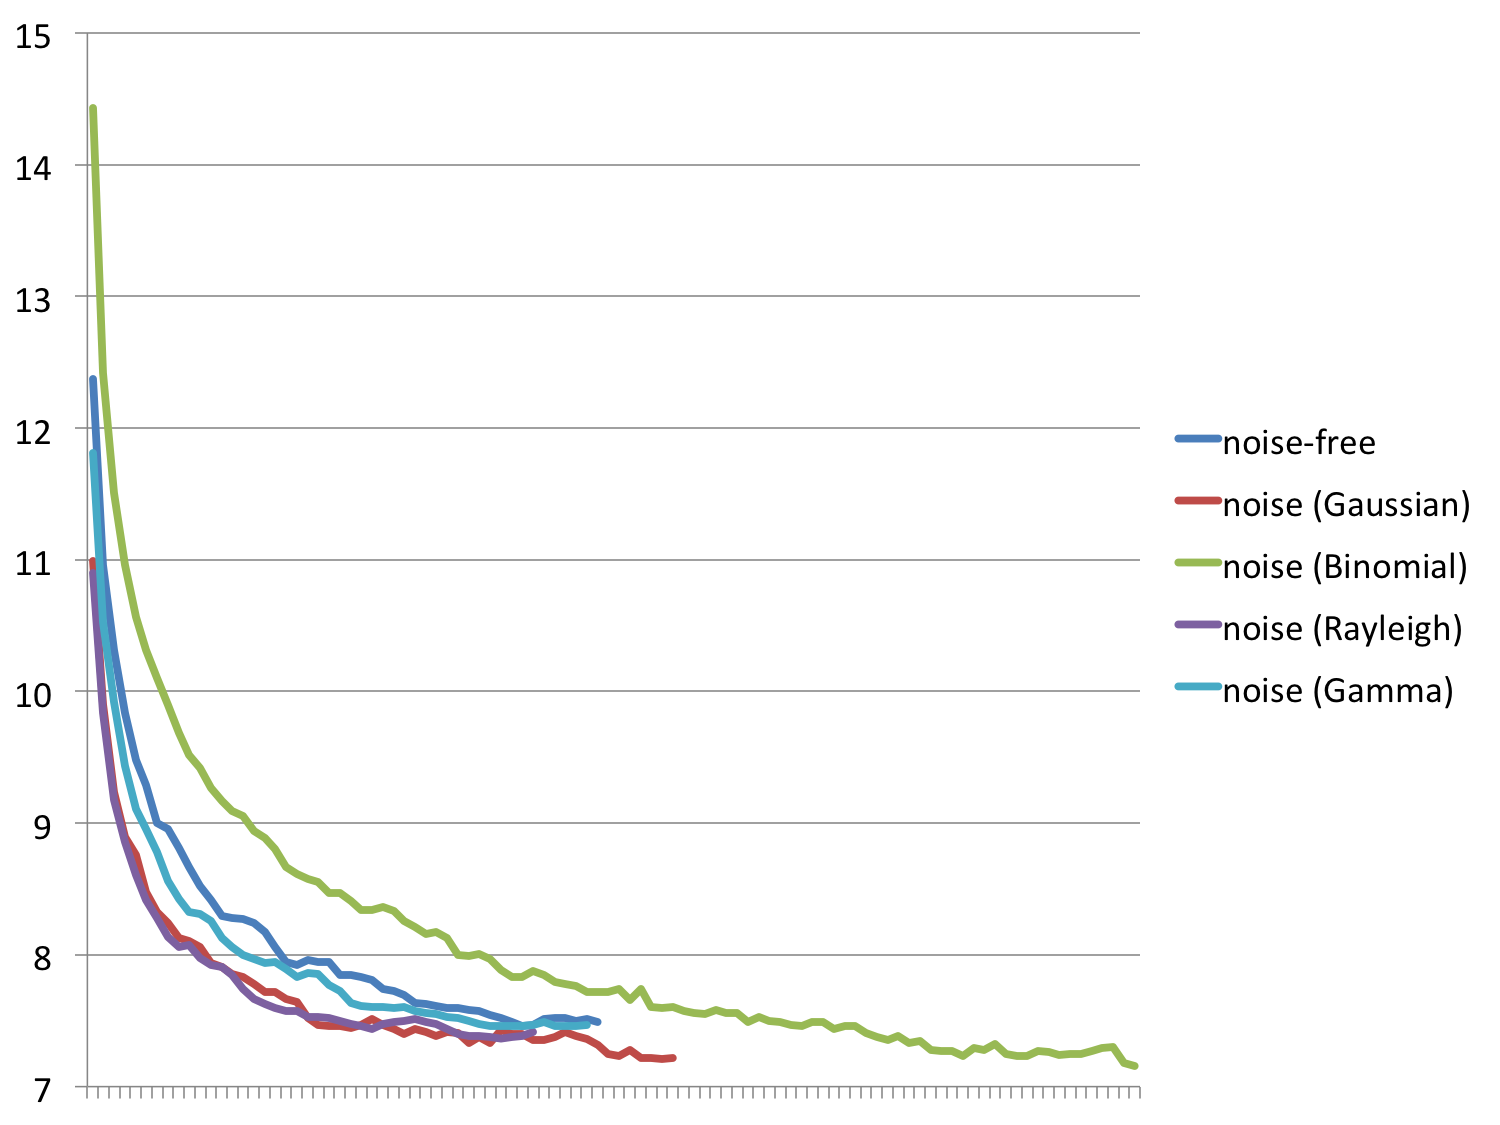
\includegraphics[width=295pt]{f-figs/logistic.png}
\caption{Logistic Regression with Noise on MNIST}
\label{logistic}
\end{figure}

% explain the figure

\subsection{Adding Noise into Multi-layer Logistic Regression}
Figure~\ref{mlp} shows test error rate using noise-free and noise-added
Multi-layer Logistic Regression on MNIST.
\begin{figure}[!htbp]
\centering
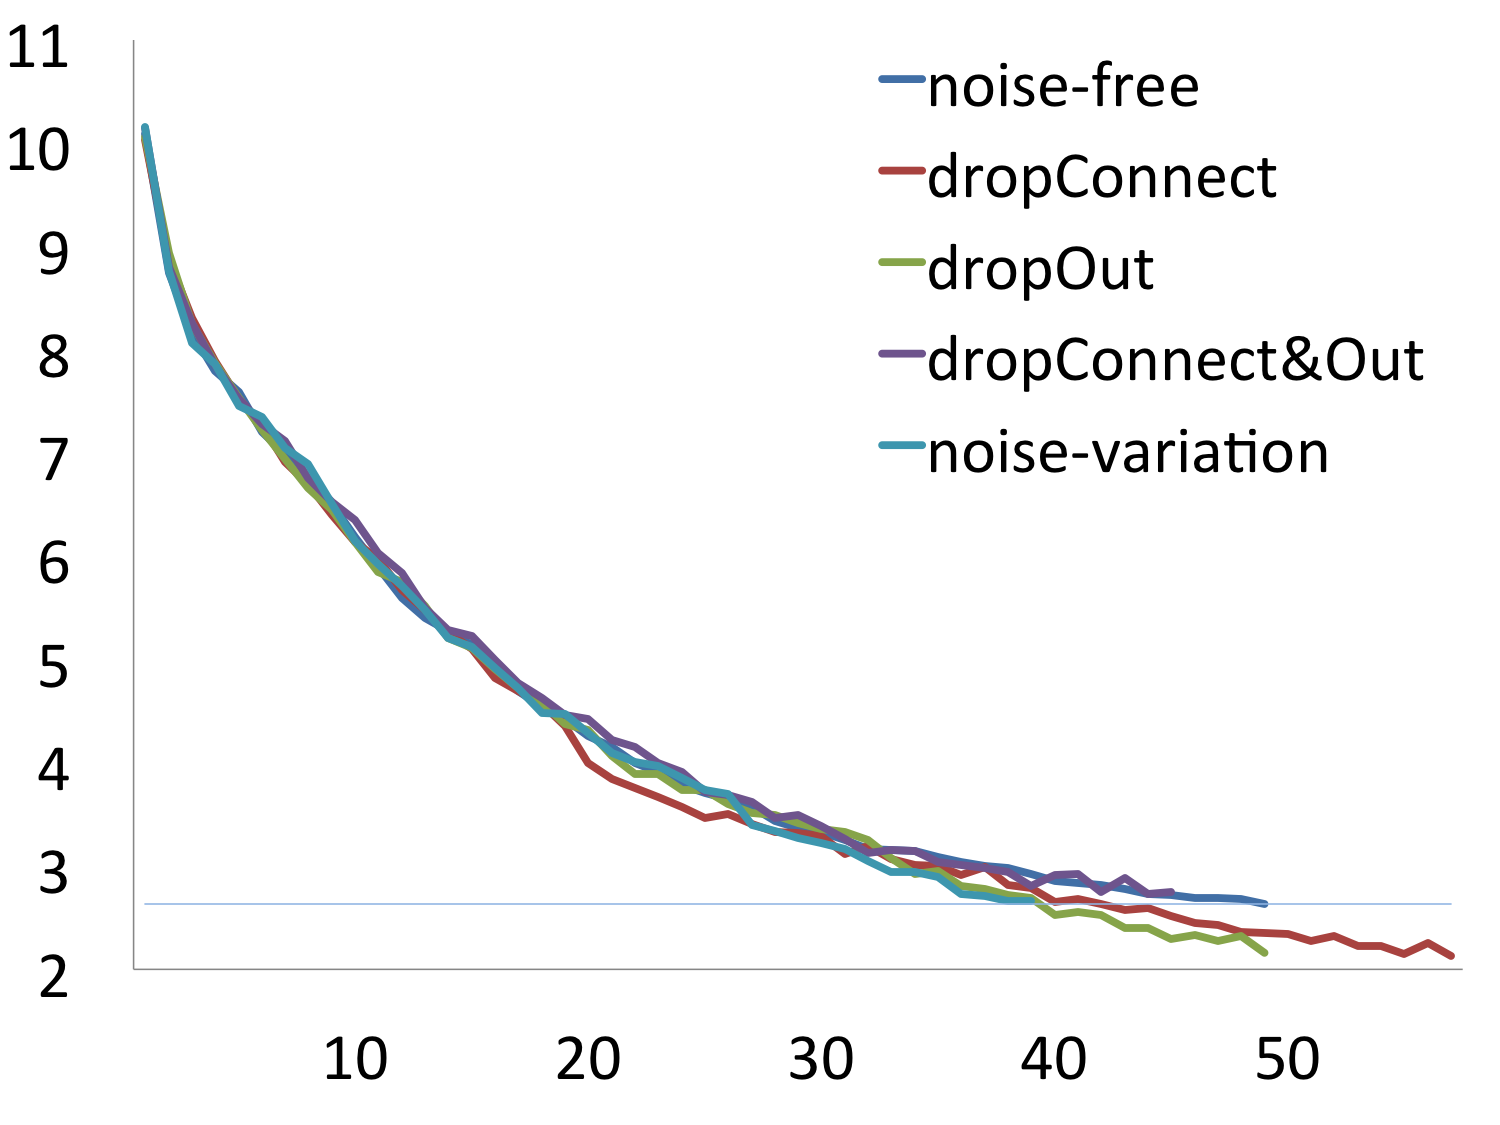
\includegraphics[width=295pt]{f-figs/mlp.png}
\caption{Multi-layer Logistic Regression with Noise on MNIST}
\label{mlp}
\end{figure}
% explain the figure

Figure~\ref{mlp10} shows test error rate using noise-free and noise-added
Multi-layer Logistic Regression on CIFAR-10.
\begin{figure}[!htbp]
\centering
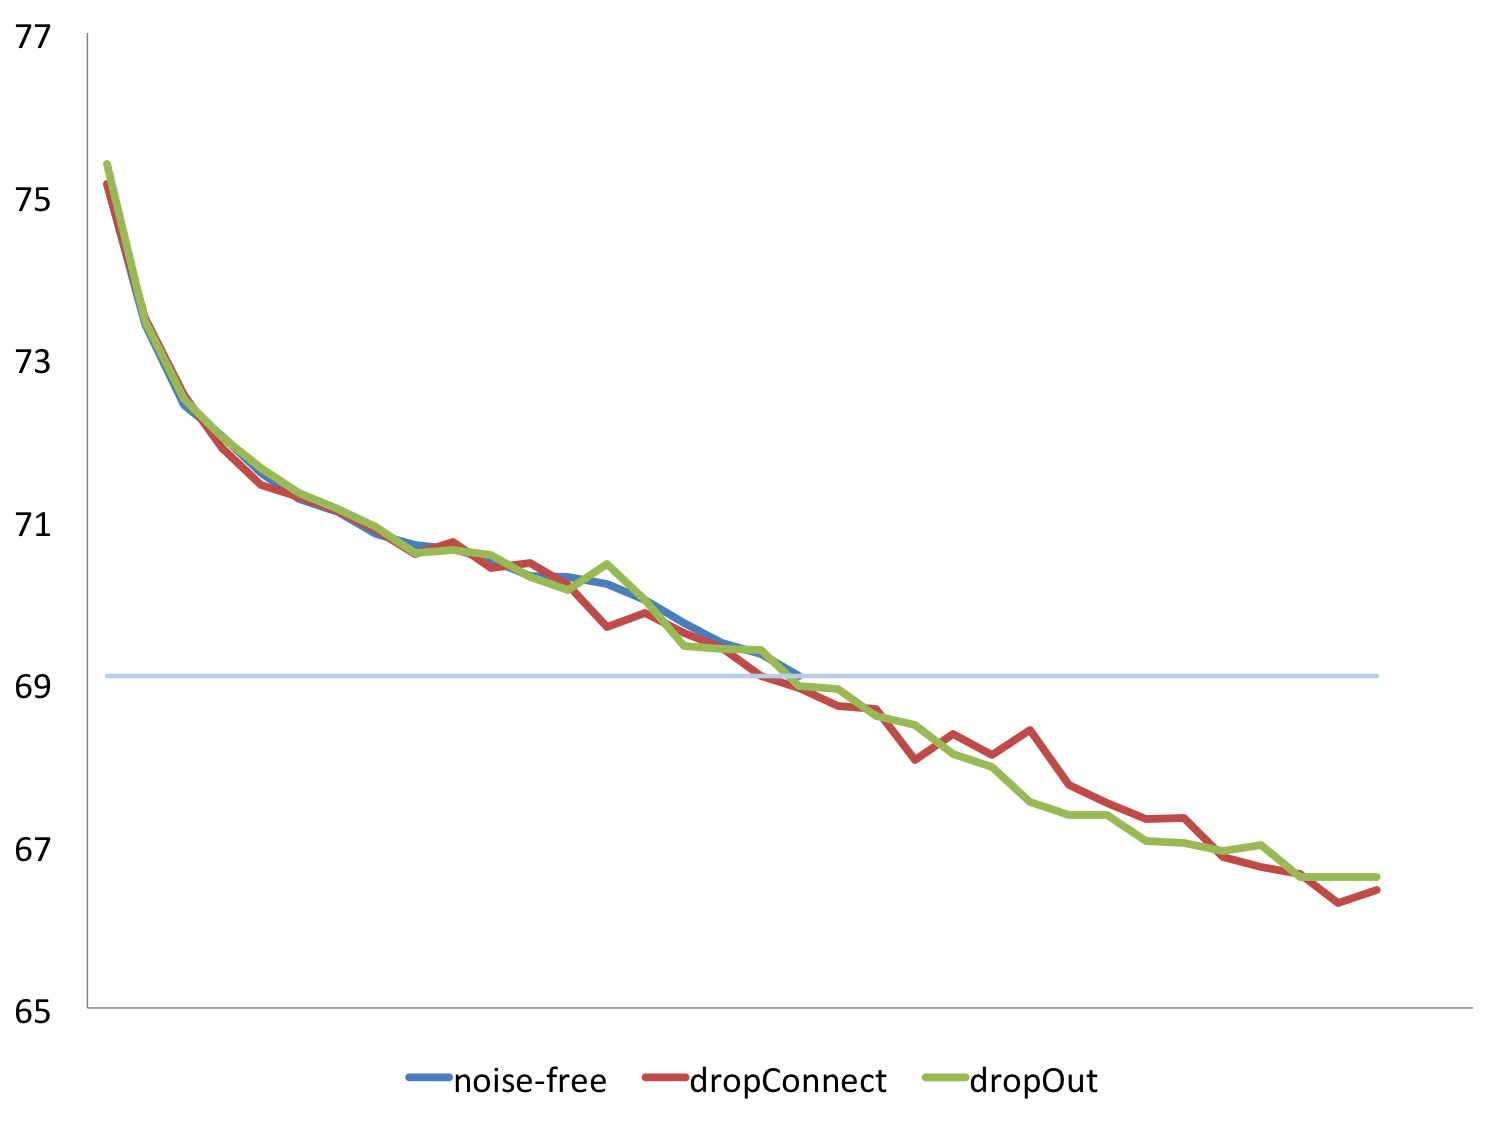
\includegraphics[width=295pt]{f-figs/mlp10.png}
\caption{Multi-layer Logistic Regression with Noise on CIFAR-10}
\label{mlp10}
\end{figure}
% explain the figure

\subsection{Adding Noise into Convolutionary Neural Network}
Figure~\ref{convo} shows test error rate using noise-free and noise-added
Convolutional Multi-layer Logistic Regression on MNIST.
\begin{figure}[!htbp]
\centering
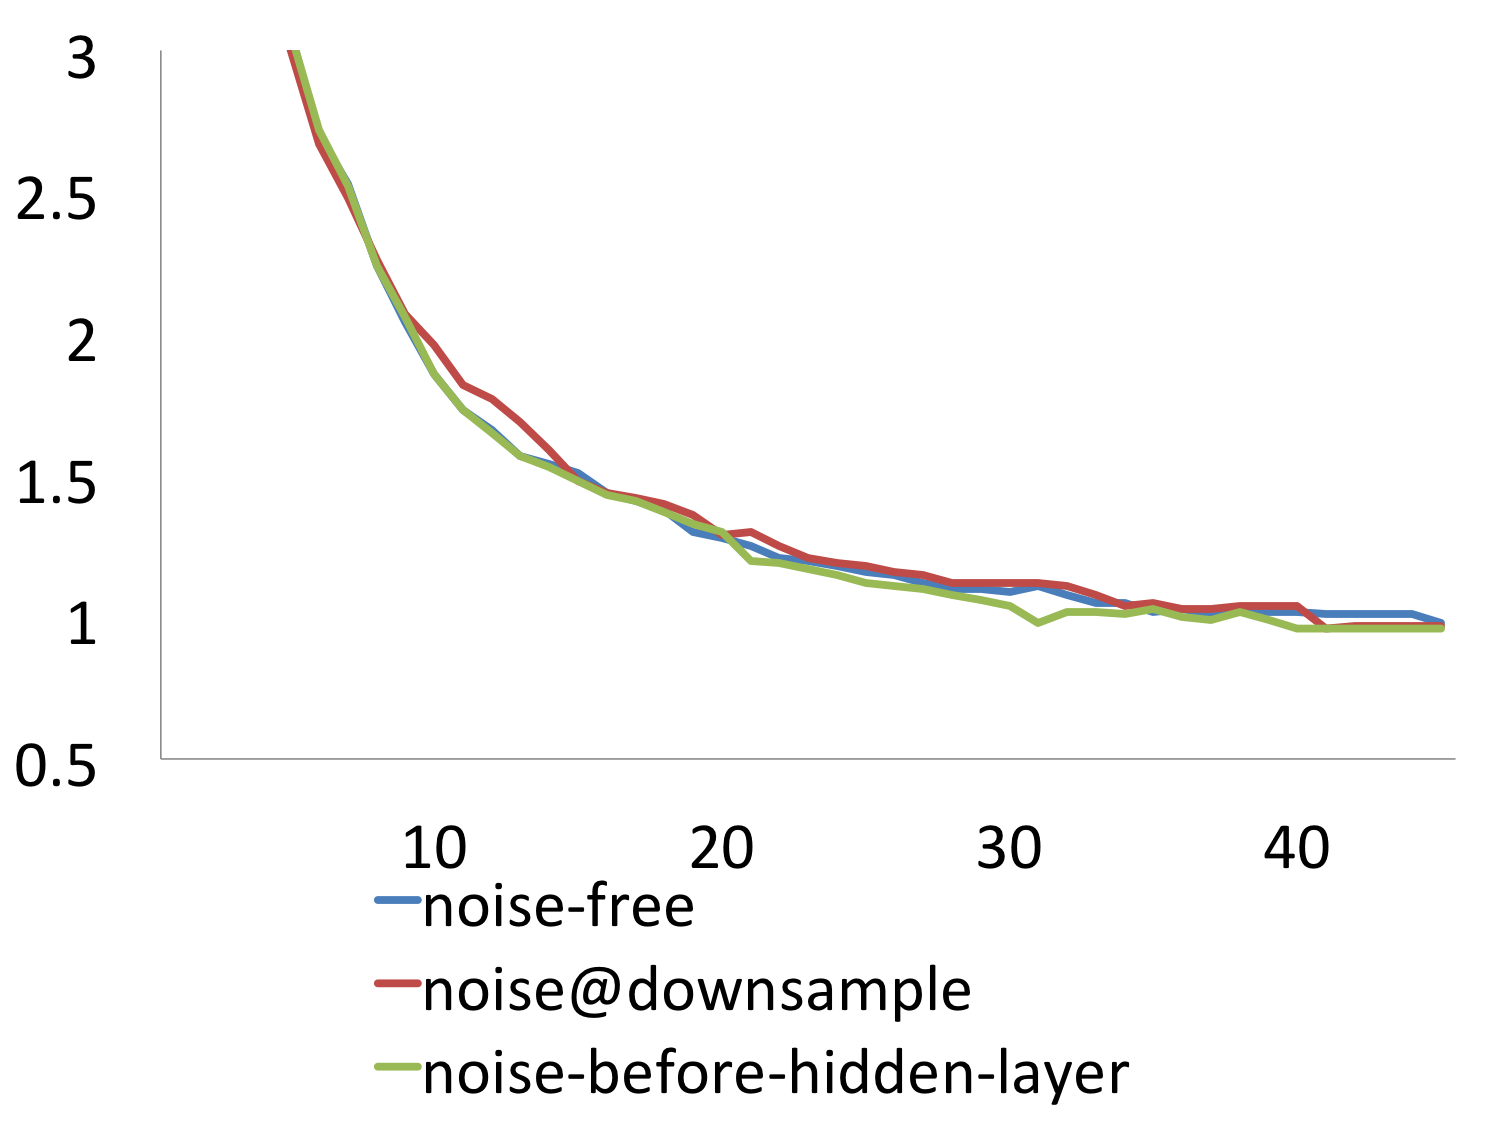
\includegraphics[width=295pt]{f-figs/convo.png}
\caption{Convolutionary Neural Network with Noise on MNIST}
\label{convo}
\end{figure}
% explain the figures

Figure~\ref{convo10} shows test error rate using noise-free and noise-added
Convolutional Multi-layer Logistic Regression on CIFAR-10.
\begin{figure}[!htbp]
\centering
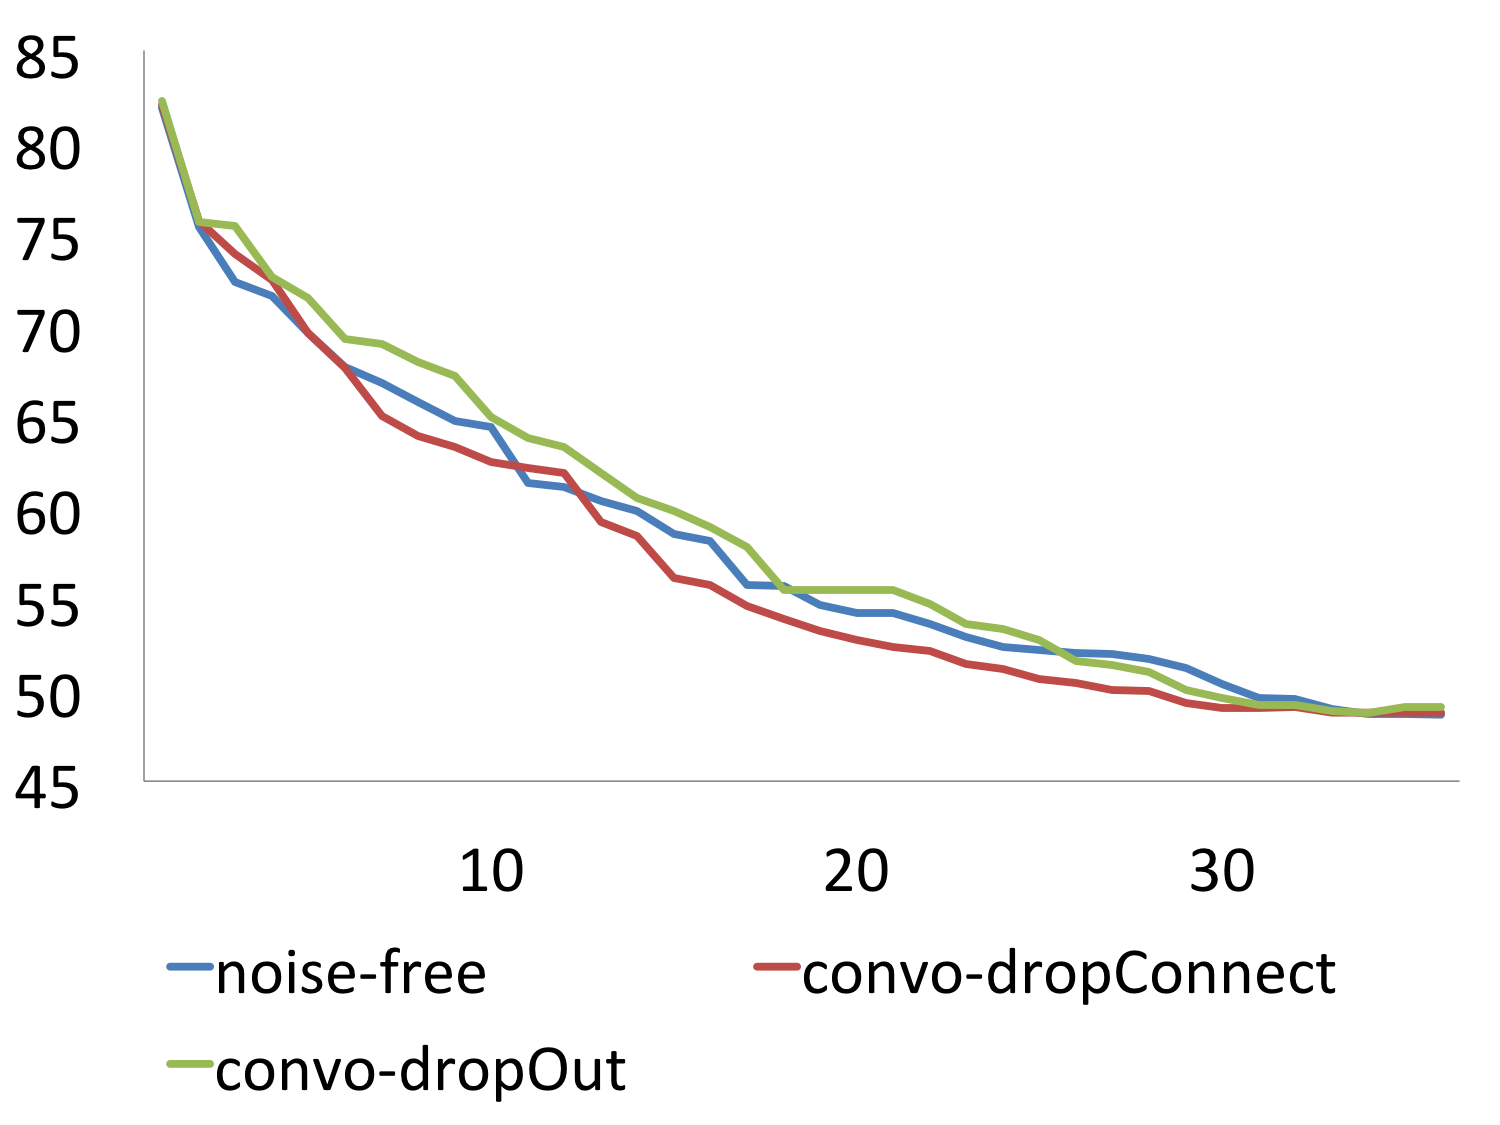
\includegraphics[width=295pt]{f-figs/convo10.png}
\caption{Convolutionary Neural Network with Noise on CIFAR-10}
\label{convo10}
\end{figure}
